\subsection{Main Features: Supervectors}

Supervectors, which have already been succesfully used in
\cite{supervectors, main} are one of the two features used in this work to train the SVM
classifier. Supervectors for a given phone are obtained by extracting the means and weights
of different
Gaussian Mixture Models derived from the adaptation of a class-independently trained GMM
to each of the instances.

So in order to go into more details of the supervectors features, a brief introduction to
GMMs is provided along with an explanation of the adaptation process.

\subsubsection{Gaussian Mixture Model}

Gaussian Mixture Model is a parametric probability density function represented as a weighted
sum of Gaussian component densities. GMMs are often used in biometric systems, specially
in speaker recognition systems, due to their ability to represent a large class of sample
distributions. One of the powerful attributes of the GMM is to form smooth approximations to
arbitrarily shaped densities \cite{gmm_reynolds}.

The densitiy function of a GMM is defined as:

\begin{equation}
  p(x) = \sum_{k=1}^{K}\pi_{k} \mathcal{N}(x|\mu_{k},\,\Sigma_{k})
\end{equation}

Each Gaussian density $\mathcal{N}(x|\mu_{k},\,\Sigma_{k})$ is called a component of the mixture
and has its own mean $\mu_{k}$ and variance $\Sigma_{k}$. The parameters $\pi_{k}$ are called
mixing coefficients and they can be thought of as the prior probability of picking the $k^{th}$
component \cite{gmm_bishop}.

In this work, GMMs are used to model the acoustic features mentioned in the previous section:
MFCCs (13), plus deltas (13) and double deltas (13). So the features for our GMMs are
39-dimensional vectors corresponding to each frame of each instance of a given phone.

It is desirable, when possible, to transform the feature space into a normally distributed feature
space because it leads to more robust results. For that reason, the acoustic features are
standardized by removing the mean and scaling to unit variance before training the GMMs.

\subsubsection{Universal Background Model Adaptation}

As in the previous works of the current line of investigation
\cite{detection_phone_level_mispronunciation_learning, main},
the GMMs are derived by the adaptation of a \textit{Universal Background Model} (UBM)
\cite{ubm_adaptation}, a technique that has been effective on significantly improving
accuracy in the speaker recongition field.

The UBM is a large class-independent GMM intended to represent the class-independent distribution
of the features. In a GMM-UBM system, the GMM is derived by adapting the parameters of the UBM
to a vector of instances with a \textit{Maximum a Posteriori} (MAP) estimation. This provides a
tighter coupling between the generated models that produces better performance than using
decoupled models such as class-dependent GMMs. In addition, it can be specially useful when
just a small number of training instances is available.

The method described in \cite{ubm_adaptation} involves adapting weight, mean and variance of each
mixture, though in the current work only weights and means are adapted because of the limited
size of the dataset. For each gaussian $k$ composing the GMM-UBM, the weight and mean parameters
are updated according to the following equations:

\begin{equation}
  \pi_{k}^{new} = [\alpha_{k} \pi_{k}^{'} + (1-\alpha_{k}) \pi_{k}]\gamma
\end{equation}

\begin{equation}
  \mu_{k}^{new} = \alpha_{k} E_{k}(x) + (1-\alpha_{k})\mu_{k}
\end{equation}

where $\pi_{k}$ and $\mu_{k}$ are the original values of the weight and mean of the
k\textsuperscript{th} component of the GMM-UBM, \mbox{$\pi_{k}^{'}$ and $E_{k}(x)$} are
the estimated values for the weight and mean calculated on the vector of instances provided
for the adaptation and the scale factor $\gamma$ is computed over all the
adapted mixture weights to ensure they sum to unity. $\alpha_{k}$ is an adaptation
coefficient that controls the balance between old and new estimates, and depends on the value of
a relevance factor input parameter $r$. A higher value of $r$ produces a decrease in the value
of $\alpha_{k}$, thus adapting in a more conservative way by assigning more importance
to the previous values. By contrary, a lower value of $r$ produces an increment in the value
of $\alpha_{k}$, thus leading to a more aggresive adaptation strategy by assigning more importance
to the new values. % No menciono que la cantidad de instancias también se relaciona con \alpha_{k}
% porque para el caso de nuestra tesis no es tenido en cuenta (relevance_factor = 0)

\subsubsection{Supervectors computation}

In order to compute the supervectors for a given phone, which are then used to train the SVM
classifier, the following steps are performed:

\begin{enumerate}
  \item At first, a GMM-UBM is trained on the acoustic features (13 MFCCs plus deltas and double
  deltas) of all the available training instances for that phone, regardless of their class.
  \item After that, an individual MAP adaptation process is carried out for each
  of the $N$ training intances, thus generating $N$ different GMMs.
  % \item The supervector generated for the i\textsuperscript{th} instance is obtained by stacking
  % the means and the weights of each of the gaussians composing the i\textsuperscript{th} GMM.
  \item Finally, for each of the training instances $i$ the supervector is obtained by stacking
  the means and the weights of each of the gaussians composing the GMM obtained from the
  i\textsuperscript{th} instance.
\end{enumerate}

The supervector computation process for a given phone instance
is summarized in the figure shown below:

\begin{figure}[H]
  \centering
  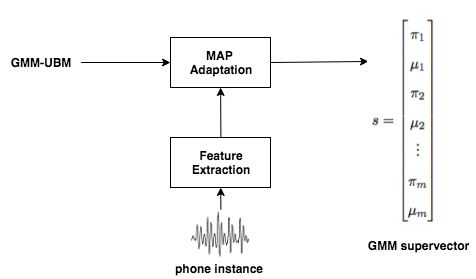
\includegraphics[width=0.6\textwidth]{files/figures/method/supervectors_extraction}
  \caption{
    Adapted figure from Campbell, Sturim, Reynolds, Solomonoff 2006 \cite{supervectors}.
    A MAP Adaptation of a GMM-UBM with $m$ gaussians
    is performed using the acoustic features of a phone instance.
    The resulting supervector is made up of the stacked weights $\pi_{i}$ and means
    $\mu_{i}$ $\forall \ 1 \leq i \leq m$, where each weight is a real value and each
    mean is a 39-dimensional vector.
  }
\end{figure}

As each derived GMM has the same number of gaussian components as the GMM-UBM, then the dimension
of each supervector is: $39*m + m$, where $m$ is the number of gaussians of the GMM-UBM. The
first term corresponds to the means while the second one to the weights.

% Intentar relacionarlo después con la parte de SVM
% The GMM supervector can be thought of as a mapping between an utterance and a
% high-dimensional vector.

Supervectors for testing are calculated following the same procedure as for training except for
the first step: the same GMM-UBM obtained in training is used for the adaptation process of the
testing instances.
